% ! TeX root = ../thesis-main.tex
%----------------------------------------------------------------------------------------
\chapter{Background}
\label{chap:background}
%----------------------------------------------------------------------------------------
This chapter describes the two main driving factors for a complete re-design of ScaFi, which are the \ac{XC} and Scala 3.
%
On one hand, \ac{XC} opens the way for considerable design improvements given the simpler set of foundational constructs it requires, consisting of the single primitive \texttt{exchange}, from which the entire language takes its name.
%
Additionally, it provides new opportunities for aggregate program developers, enabled by the expressiveness of \ac{XC}, regarding, in particular, the possibility of sending differentiated messages to neighbors using the \texttt{exchange} primitive\cite{xc}.
%
On the other hand, Scala 3 introduces significant breaking language changes and improvements from Scala 2, nevertheless featuring binary retro-compatibility.
%
This promotes the rewriting of Scala 2 libraries in a way that exploits the new language features while providing cross-builds to Scala 2 enabled by the Scala 3 compiler \quotes{Dotty}\footnote{\url{https://github.com/lampepfl/dotty}}.

\section{The Exchange Calculus}\label{chap:background->sec:xc}

\ac{XC} is a language that formalizes a tiny set of key mechanisms, sufficient to express the overall behavior of a distributed collective adaptive systems in a declarative fashion\cite{xc}.
%
\ac{XC} offers both an operational semantics, defining the local interpretation of these mechanisms on each device, and a denotational semantics, which provides an interpretation of these mechanisms at the network level, abstracting away the operational semantics details.
%
Therefore, operational semantics guides the implementation of \ac{XC} as a framework, while denotational semantics is the sole knowledge base necessary when programming a \ac{CAS} with this language.
%
The \ac{XC} language generalizes over \ac{FC} and is derived from the typed lambda calculus\cite{xc}.

The building blocks of \ac{XC} are:
\begin{itemize}
    \item the basic system model and its assumptions;
    \item the data type for neighboring values, \textit{NValues};
    \item the only communication primitive, \texttt{exchange};
    \item the concept of \textit{alignment}.
\end{itemize}

For the expressiveness of \ac{XC}, two crucial factors are:
\begin{itemize}
    \item the ability, for an \textit{exchange} invocation, to send differentiated messages to neighbors,
    \item and \textit{alignment}, because it enables \textit{functional composition of distribute behavior}\cite{xc}.
\end{itemize}

\subsection{System model}

Similarly to \ac{FC}, \ac{XC} targets a system modeled as a collection of devices, generally equipped with sensors and/or actuators, that repeatedly compute execution \textit{rounds} of the \textbf{same program} and exchange asynchronous \textit{messages} with their respective neighbors\cite{xc}.
%
In this environment, a device can fail, reboot, experience network outages, and dynamically change neighbors.
%
At each execution round, a device independently gathers a local context, consisting of inbound messages from neighbors, sensors data, and memory of its previous round of execution, if any, and then \textit{atomically executes} the \ac{XC} program common for all the devices, acting on its local context\cite{xc}.
%
The program can result in an output, that comprises side effects such as actuation, as well as, implicitly, the messages to send to neighbors for coordination\cite{xc}.
%
At the end of each round, a device begins waiting for an arbitrary time lapse, during which the device is considered \quotes{sleeping}.
%
After the sleep time, the device \quotes{wakes up} and begins the next execution round\cite{xc}.
%
During sleep, a device must still collect inbound messages and apply two policies: \textit{last-message buffering} and \textit{last-message dropping}.

\paragraph{Last-message buffering} means that every message received by a device is collected in a buffer and kept until some established criterion determines its \textit{expiration}, even across multiple execution rounds\cite{xc}.
%
As a result, the message expiration is also the minimum time that a device takes to realize that a neighbor has disappeared, either because of a failure or a neighbor network change.

\paragraph{Last-message dropping} means that every message received by a device supersedes the last message, still in the buffer, coming from the same device.\cite{xc}
%
This implies a notion of identity of devices, which is a way to recognize a neighbor's identity to discard obsolete messages coming from them.

\paragraph{Communication between devices} defined in \ac{XC} is agnostic of the message exchange medium, channel, network topology, or discovery mechanisms.
%
Messages in such a model are subject to classic distributed systems communication properties, such as unpredictable delays and drops\cite{xc}.
%
Additionally, for \ac{XC} and its implementations, a device memory of its previous execution round result can be considered a self-message at all effects.
%
This consideration models a reboot, which in practice is a memory loss, to a self-message drop, thus simplifying the device model in the operational semantics.

\subsection{NValues} \label{chap:background->sec:xc->subsec:nvalues}

\ac{XC} features two kind of values, \textit{local values} and \textit{neighbouring values} (NValues or nvalues).
%
Local values $l$ refer to all the traditional types \texttt{A} like integer, float, list, and so on.
%
NValues, instead, are a map $\underline{\mathbf{w}}$ from device identifiers $\delta_i$ to local values $l_i$, with a default local value $l$, written $l[\delta_1 \mapsto l_1, ..., \delta_n \mapsto l_n]$\cite{xc}.

NValues refer to values coming from neighbors, which, in highly decoupled distributed systems, almost always consist of a subset of all devices, for example, because all other devices are out of reach in a spacial-dependent neighboring relationship.
%
The default value is used when evaluating a NValue $\underline{\mathbf{w}} = l[\delta_1 \mapsto l_1, ..., \delta_n \mapsto l_n]$ for a given $\delta_i$ with $\delta_i$ not present in $\underline{\mathbf{w}}$.
%
The notation above can thus be read as \quotes{the nvalue $\underline{\mathbf{w}}$ is $l$ everywhere (i.e. for all neighbors) except for devices $\delta_1, ..., \delta_n$ with values $l_1, ..., l_n$, respectively}\cite{xc}.

For example, in \cref{fig:xc-nvalues-exampke}, the device $\delta_2$ wakes up for computation $\epsilon_2^4$ and processes a nvalue $\underline{\mathbf{w}} = 0[\delta_1 \mapsto 5, \delta_3 \mapsto 4, \delta_4 \mapsto 2]$, which corresponds to the messages carrying the scalar values 5, 4, and 2 sent by devices $\delta_1$, $\delta_3$, and $\delta_4$, respectively, some of which while device $\delta_2$ was asleep.
%
For all other devices, the entry in $\underline{\mathbf{w}}$ evaluates to $0$.
%
After the computation, $\delta_2$ sends out the messages represented by $\underline{\mathbf{w'}} = 0[\delta_1 \mapsto 7, \delta_4 \mapsto 1]$.
%
For instance, $7$ is sent to $\delta_1$, $1$ to $\delta_4$, and $0$ to all other neighbors, such as $\delta_3$.
%
Evaluation of a nvalue for a given $\delta'$ can be noted as $\underline{\mathbf{w}}(\delta')$ and its result is the local value $l'$ if $\delta' \mapsto l'$ is in $\underline{\mathbf{w}}$, or else the default value $l$ of $\underline{\mathbf{w}}$.
%
For $\underline{\mathbf{w'}}$, $\underline{\mathbf{w'}}(\delta_1)$ is $7$, and $\underline{\mathbf{w'}}(\delta_3)$ is 0.
%
Another notation used in the paper is $\underline{A}$, to indicate the type of a nvalue $\underline{\mathbf{w}} = l[\delta_1 \mapsto l_1, ..., \delta_n \mapsto l_n]$ where $l_1, ..., l_n$ are of type $A$\cite{xc}.

NValues generalize local values, in the sense that a local value $l$ with type $A$ can be automatically converted to a nvalue $l[]$ with type $\underline{A}$, with $l$ as the default value for every device\cite{xc}.
%
This simplifies the formalization of \ac{XC}, where local values and nvalues are treated uniformly\cite{xc}.
%
The same principle can be applied to functions, which can be implicitly lifted to operate on nvalues, by applying them on the content of the maps pointwise, using the default values where necessary\cite{xc}.
%
For example, given $\underline{\mathbf{w_1}} = 1[\delta_1 \mapsto 2, \delta_3 \mapsto 4]$ and $\underline{\mathbf{w_2}} = 3[\delta_1 \mapsto 5, \delta_2 \mapsto 6]$, $\underline{\mathbf{w_3}} = \underline{\mathbf{w_1}} + \underline{\mathbf{w_2}} = 4[\delta_1 \mapsto 7, \delta_2 \mapsto 7, \delta_3 \mapsto 7]$.
%
Another example is $\underline{\mathbf{w_4}} = \underline{\mathbf{w_1}} + 1 = 2[\delta_1 \mapsto 3, \delta_3 \mapsto 5]$, which uses the automatic promotion of $1$ to $1[]$.

NValues can be folded over, using the built-in function $nfold(f : (A, B) \rightarrow A, \underline{\mathbf{w}} : \underline{B}, l : A) : B$, which takes an accumulator function $f$ repeatedly applied to neighbors' values in a nvalue, excluding the value for the \textit{self} device, starting from a base local value $l$, and using the default value of $\underline{\mathbf{w}}$ for neighbors not present in the map\cite{xc}.
%
For example, given a device $\delta_1$ performing a $nfold$ operation on $\underline{\mathbf{w}} = 3[\delta_1 \mapsto 10, \delta_2 \mapsto 1, \delta_3 \mapsto 2]$ while the current set of its neighbors is $\{\delta_3, \delta_4\}$, then $nfold(+, \underline{\mathbf{w}}, 1) = 6$.
%
Given that nvalues are agnostic to the ordering of elements, i.e. the ordering of device identifiers in the map, $f$ is assumed to be associative and commutative\cite{xc}.

\begin{figure}
    \centering
    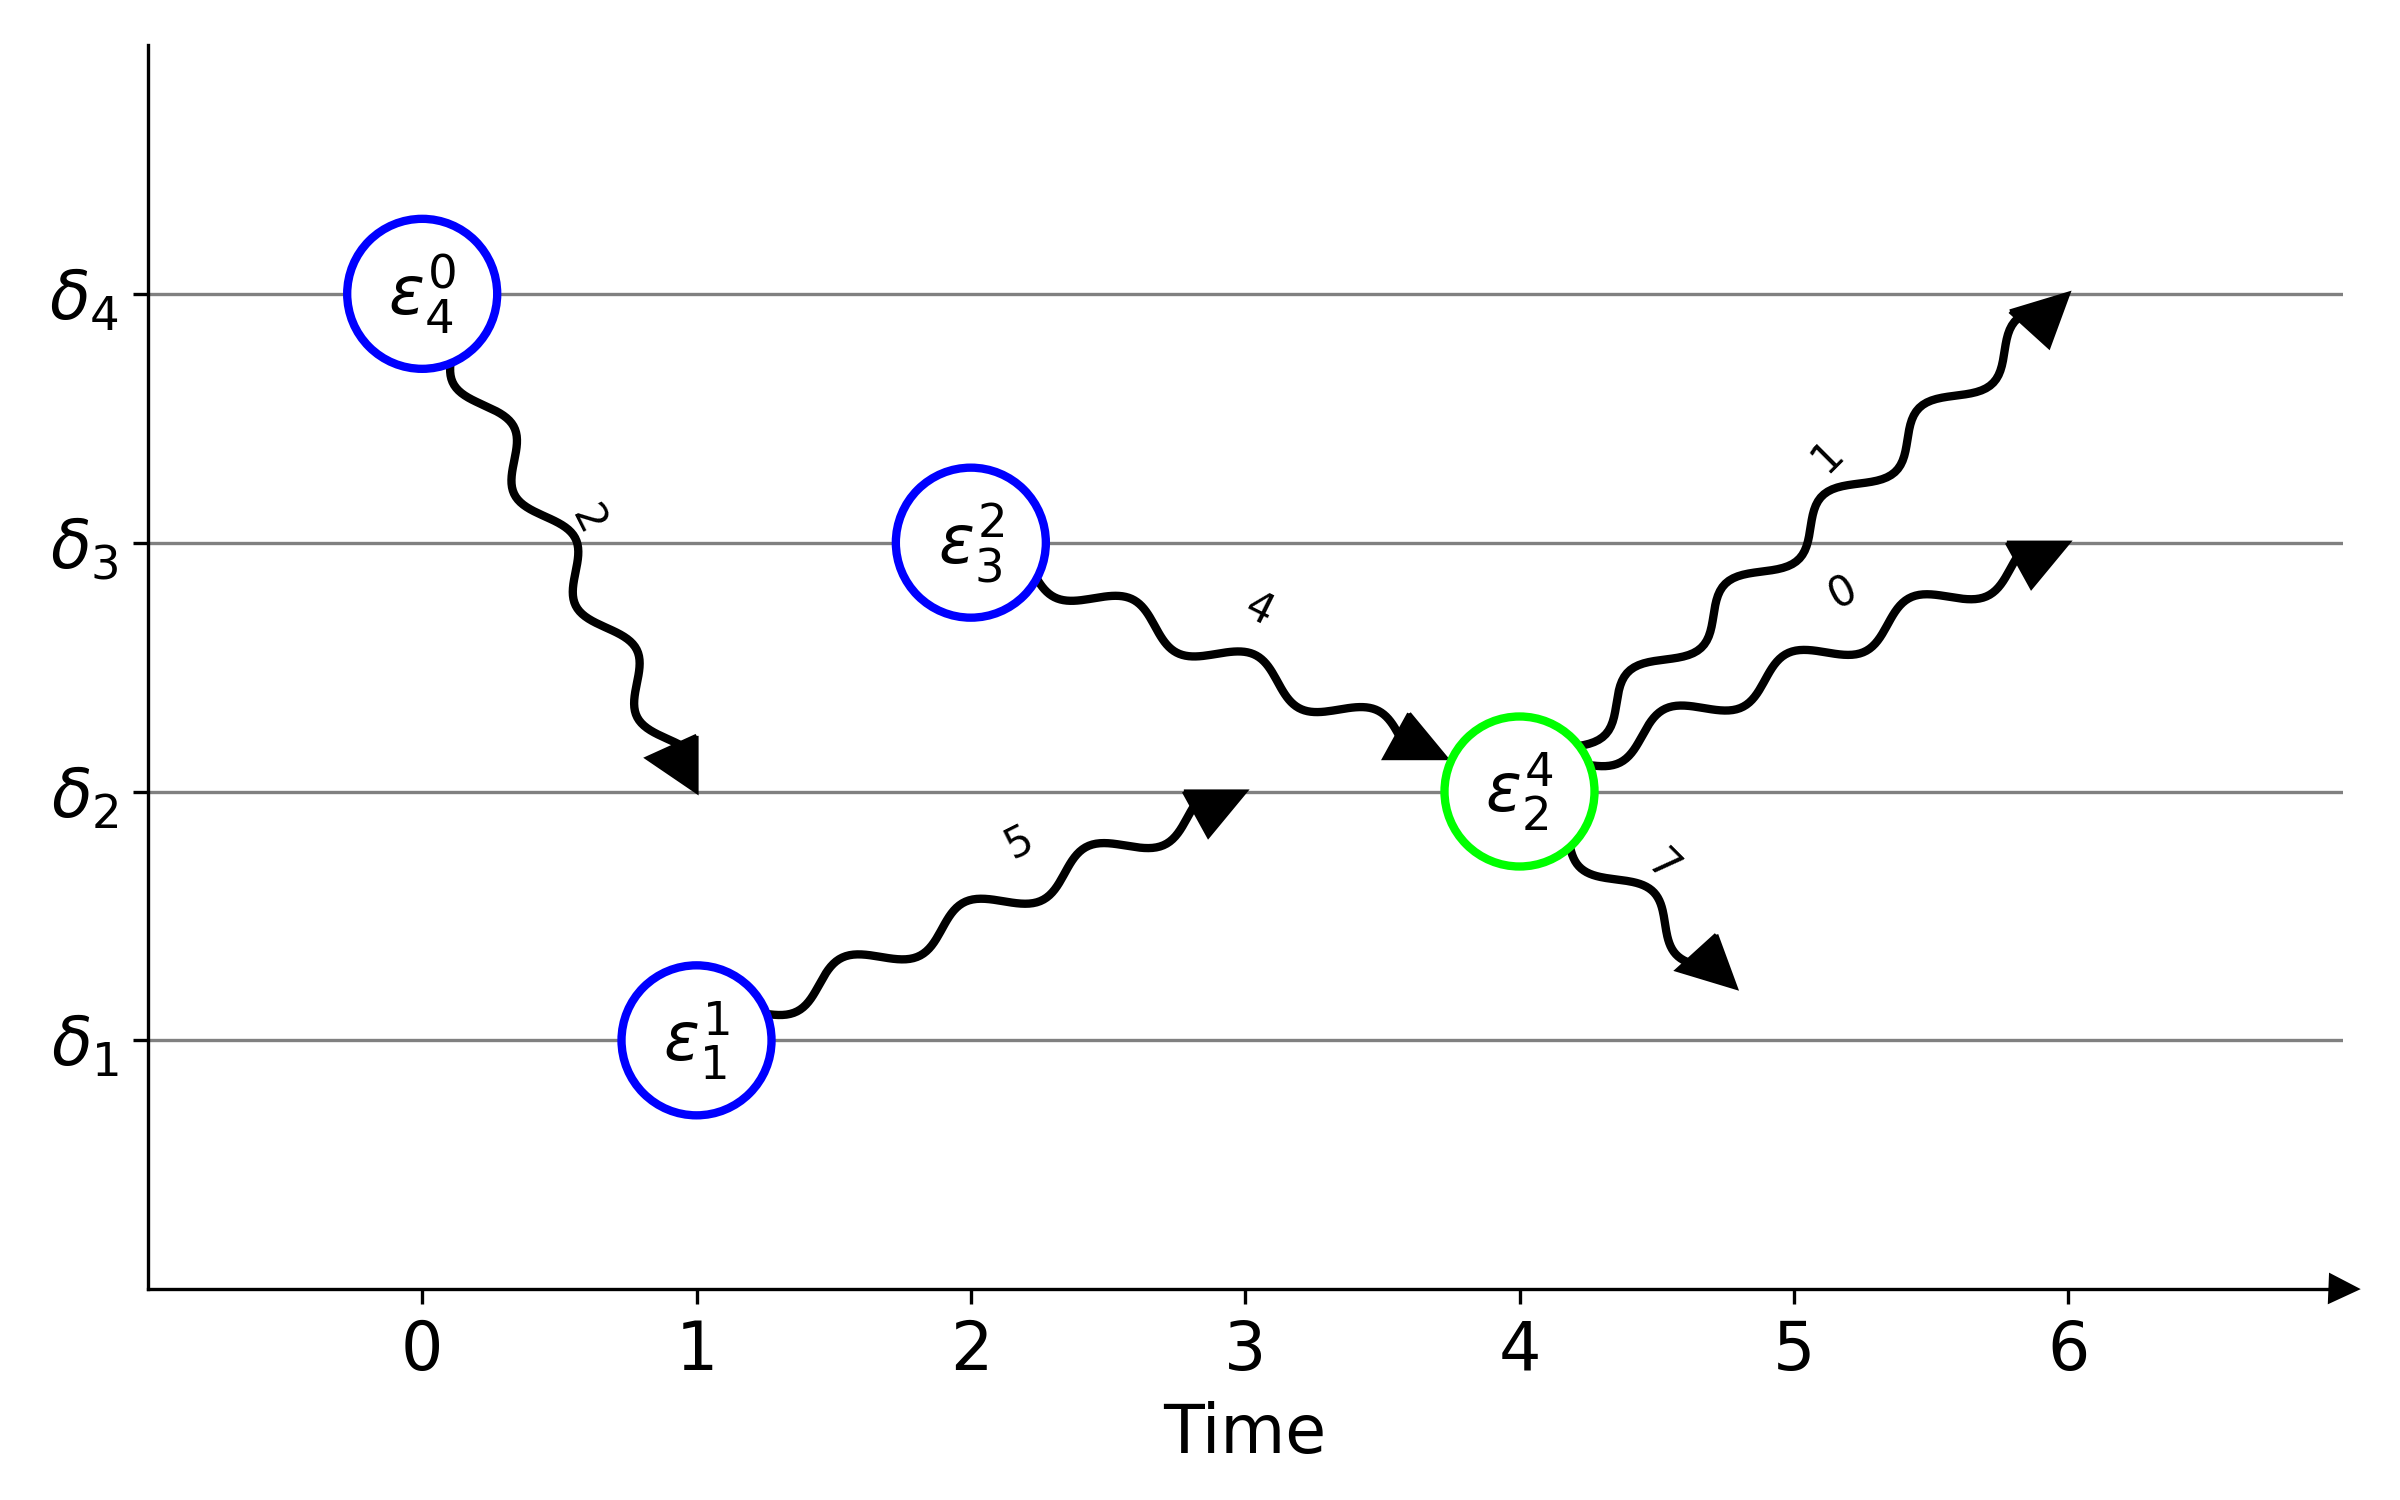
\includegraphics[width=.8\linewidth]{figures/nvalues-example.png}
    \caption{\ac{XC} system model, from the point of view of the wake-up event $\epsilon_2^4$ pictured in green.}
    \label{fig:xc-nvalues-exampke}
\end{figure}

\paragraph{Additional built-in operations} on nvalues are $self(\underline{\mathbf{w}} : \underline{A}) : A$ which returns the local value $\underline{\mathbf{w}}(\delta)$ for the self device $\delta$, and $updateSelf(\underline{\mathbf{w}} : \underline{A}, l : A) : \underline{A}$ which returns a new nvalue with the same content of $\underline{\mathbf{w}}$ but with the value for the self device replaced by $l$\cite{xc}.
%
Given the built-in function $uid$ that returns the device identifier of the self device, the following property holds: $self(\underline{\mathbf{w}}) = \underline{\mathbf{w}}(uid)$.
%
The complete syntax for \ac{XC} is available in the original paper\cite[p. 4]{xc}.

\subsection{The \texttt{exchange} primitive}

The following description is based on the original paper for \ac{XC}\cite{xc}.
%
The only communication primitive present in \ac{XC} is the function $$exchange(e_i, (\underline{\mathbf{n}}) \Rightarrow \mathbf{\return} e_r \mathbf{\send} e_s)$$ which is defined using syntactic sugar and translates to $$exchange(e_i, (\underline{\mathbf{n}}) \Rightarrow (e_r, e_s))$$
%
The evaluation of the primitive follows three steps:
\begin{enumerate}
    \item the device evaluates the expression $e_i$ to obtain the \textit{initial} local value $l_i$;
    \item $\underline{\mathbf{n}}$ is substituted with the nvalue $\underline{\mathbf{w}}$ of messages received from neighbors for this exchange, using $l_i$ as the default value for $\underline{\mathbf{w}}$, and the device evaluates the expression $e_r$ to the value $v_r$ to be returned;
    \item the device evaluates the expression $e_s$ to obtain a nvalue $\underline{\mathbf{w_s}}$ to be sent to neighbors such as $\delta'$, that will use their corresponding value $\underline{\mathbf{w_s}}(\delta')$ in their next execution round.
\end{enumerate}

As a shorthand, $$exchange(e_i, (\underline{\mathbf{n}}) \Rightarrow \mathbf{\return} e \mathbf{\send} e)$$ can be written as $$exchange(e_i, (\underline{\mathbf{n}}) \Rightarrow \mathbf{\retsend} e)$$ according to the \ac{XC} paper\cite{xc}.

Two examples of reusable functions written in \ac{XC} can be seen in \cref{lst:xc-program}.
%
There, $mux(cond, e_1, e_2)$ is a conditional expression that first evaluates $cond$, $e_1$, and $e_2$, and then returns the value of $e_1$ if $cond$ is true, or the value of $e_2$ otherwise.
%
\texttt{mux} is useful to avoid breaking the alignment of the network by using conditionals, as explained in \cref{chap:background->sec:xc->subsec:alignment}.
%
In the examples, $\underline{senseDist}$ is a network-based sensor that returns the nvalue containing the distances to neighbors, abstracting over the way the device obtains the measurements, with $Infinity$ as its default value used for all other devices.
%
\texttt{distanceEstimate} computes the minimum distance from a source using the distance sensor and the neighbors estimate $\underline{\mathbf{n}}$ of their minimum distance from the same source.
%
\texttt{distanceTo} computes the minimum distance from a source determined by a boolean expression, which is a \textit{gradient} with value $0$ in all devices where $src$ is true, and the minimum distance from the source in all other devices connected to a source device, or else $Infinity$.

\lstinputlisting[float,language=XC,label={lst:xc-program}, caption={Implementation of a network-wide gradient, called \texttt{distanceTo}, in \ac{XC}.}]{listings/xc-gradient-distance.xc}

\subsection{Alignment}\label{chap:background->sec:xc->subsec:alignment}

A program can execute multiple exchanges in a single round, and \ac{XC} ensures that messages are dispatched to corresponding exchange expressions, using the concept of \textit{alignment}.
%
The corresponding exchange expressions are those that are found in the same position in the \ac{AST} and the same stack frame, thus ensuring correct alignment in case of branches, function calls, and recursion\cite{xc}.
%
As a consequence, the evaluation of an aggregate program implicitly builds a tree representation, which all aligned devices, as well as the device itself in the next rounds, replicate.

Conditionals such as $if (cond) {e_1} else {e_2}$ interfere with alignment because only the \texttt{exchange} operations in the same position within the AST and stack frame align\cite{xc}.
%
As a consequence, \texttt{exchange} only aligns across devices that take the same branch of all the conditionals that are parent of the \texttt{exchange} operation in the AST.

Alignment controls the evaluation of sub-expressions, in particular the evaluation of expressions involving nvalues, because in such expressions only aligned neighbors are considered.
%
As a result, every \texttt{if} expression splits the network into two non-communicating sub-networks, each evaluating a different branch based on the condition\cite{xc}.
%
Isolated sub-networks in this regard are also called \textit{sub-domains}, or simply \textit{domains}.

\subsection{Formalization of XC}

\ac{XC} is formalized in the paper\cite{xc} in its syntax, operational semantics, and denotational semantics.
%
The language takes inspiration from \ac{ML}, and as such is a standard functional language with a classic Hindley-Milner type system, whose formalization makes \ac{XC} type sound and deterministic once extended with \textit{value-tree} typing and \textit{configuration} typing\cite{xc}.

\subsection{Implementing FC primitives with exchange}

With the implementation of \ac{FC} primitives and expressiveness using \ac{XC}, the \ac{XC} inherits all the results found in literature that hold for \ac{FC}, such as eventual recovery and stabilization after transient changes\cite{self-stabilisation-in-fc}, independence from the density of devices\cite{density-independence-in-fc}, real-time error tolerance and convergence\cite{real-time-error-tolerance-in-fc}, and the list continues\cite{xc}.
%
Additionally, \ac{XC} opens the possibilities for writing programs not expressible with \ac{FC}, thanks to the expressiveness of the \texttt{exchange} primitive which allows sending differentiated messages to neighbors.
%
In \ac{FC}, the concept of \textit{field}, also called \textit{neighboring value}, is defined as a neighbor-dependent value consisting of a map $\phi = \overline{\delta} \mapsto \overline{l}$ from neighbors to local values, which can be promoted to nvalue with any valid default value $l$.
%
This preserves the behavior of programs written in \ac{FC} but interpreted within \ac{XC}\cite{xc}.

\ac{FC} presents three main primitives to implement with \ac{XC}:
\begin{itemize}
    \item \texttt{nbr}, used to access the neighbors values\cite{from-dc-to-fc-and-ap};
    \item \texttt{rep}, used to compute a new value of an expression based on the result of the same expression in the previous round\cite{from-dc-to-fc-and-ap};
    \item \texttt{share}, used to efficiently access neighbors' values while computing a new value from the previous result with a single primitive\cite{share-operator}.
\end{itemize}

The \texttt{nbr} primitive can be implemented as: $$nbr(e: A): \underline{A} = exchange(e, (\underline{n}) \Rightarrow \return \underline{n} \send e)$$
%
The \texttt{rep} primitive can be implemented as: $$rep(e_i: A)\{(x) \Rightarrow e_n\}: A = exchange(e_i, (\underline{x}) => \retsend e_n[x := self(\underline{x})])$$
%
The \texttt{share} primitive can be implemented as: $$share(e_i: A)\{(\underline{x}) \Rightarrow e_n\}: A = self(exchange(e_i, (\underline{x}) => \retsend e_n))$$

\section{Scala 3}\label{chap:background->sec:scala3}

Scala 3 is the latest major release of the Scala language, a high-level programming language that combines object-oriented and functional programming paradigms.
%
Scala is a statically typed, general-purpose programming language designed to express common programming patterns in a concise, elegant, and type-safe way.
%
Scala 3 is compiled using the \textit{Dotty} compiler\footnote{\url{https://github.com/lampepfl/dotty}}, which is based on the \ac{DOT} calculus\cite{dot}, while Scala 2 is compiled using the \textit{scalac} compiler\footnote{\url{https://github.com/scala/scala}}.
%
This section provides an overview of the main features of Scala 3, which are relevant for the re-design of ScaFi, while also highlighting the differences between Scala 2 and Scala 3.

\subsection{General considerations on Scala 3}

Even though Scala 3 introduces breaking changes in the syntax from Scala 2, most of the code written in Scala 2 can be compiled with Dotty and is also binary compatible with Scala 2.
%
This possibility has been exploited by the Scala community to avoid reimplementing a new standard library for Scala 3, using the Scala 2 standard library instead, rewritten to be cross-compiled for both Scala 2 and Scala 3.

Originally, Scala 2 and Scala 3 compile to \ac{JVM} bytecode, but Scala 3 also supports the \ac{JS} and \textit{LLVM} backends, which are used to compile Scala code to JavaScript and native code, respectively, thanks to community-driven projects\footnote{Scala.js at \url{https://scala-js.org}}\footnote{Scala Native at \url{https://scala-native.org}}\cite{scala-js}.
%
The provided support for cross-platform distribution, together with the popularity of Scala for distributed systems development\cite{scala-popularity} and the flexibility of the upgraded language features for advanced internal \ac{DSL} design, makes Scala 3 a great choice for a new ScaFi implementation based on \ac{XC}.

\subsection{Values in Scala}

In Scala, every value has a type, following the type hierarchy explained in \cref{chap:background->sec:scala3->subsec:type-hierarchy}.
%
When declaring a new variable or field as a container of a value, the type can be explicitly declared, or it can be inferred by the compiler.
%
Every declaration of a variable or field must be preceded by the \texttt{val} keyword for an immutable value, or the \texttt{var} keyword for a mutable value.
%
Immutable values cannot be reassigned, while mutable values can be reassigned, but the type of the value cannot be changed.
%
\texttt{val} doesn't guarantee that the value itself is immutable, but only that the reference to the value cannot be changed.


\subsection{New control syntax and significant indentation}

Scala 3 introduced a new syntax for control expressions, as well as new rules that allow the indentation alone to replace the use of curly braces.
%
Both these changes are aimed at making the code more readable and concise, sometimes noticeably closer to the natural language.
%
For example, in \cref{lst:scala2-with-braces}, the \texttt{if} expression is written with the traditional syntax, while in \cref{lst:scala3-without-braces} the same expression is written using the new syntax.
%
The same is true of the \texttt{for} expression, the \texttt{while} loop, and the \texttt{match} expression.

\lstinputlisting[float,language=Scala,label={lst:scala2-with-braces}, caption={Examples of syntax using braces in Scala 2.}]{listings/scala2-with-braces.scala}
\lstinputlisting[float,language=Scala,label={lst:scala3-without-braces}, caption={Examples of syntax avoiding braces in Scala 3.}]{listings/scala3-without-braces.scala}

In cases where a code block consists of many lines that make it a bit hard to follow indentation, the new syntax can be combined with \texttt{end} statements, as shown in \cref{lst:scala3-with-end}.

\lstinputlisting[float,language=Scala,label={lst:scala3-with-end}, caption={Example of syntax using \texttt{end} statements in Scala 3.}]{listings/scala3-without-braces-with-end.scala}


\subsection{Traits and classes}

Traits are a powerful feature of Scala that replaces Java's interfaces and abstract classes and were first introduced as a mechanism to organize behavior into small, modular units\cite{traits}.
%
In Scala, traits can be used both to define interfaces and to provide partial implementations, composable and mixable into classes when a concrete implementation is needed.
%
With Scala 3, traits are now able to have parameters like classes do, enhancing their expressiveness.
%
Additionally, Scala 3 introduces new rules for instantiation of classes that allow to avoid the use of the \texttt{new} keyword, as shown in \cref{lst:scala3-without-braces}.
%
This feature is called \textit{universal apply methods} and is enabled by the generation of \texttt{apply} methods for classes done by the compiler when the user does not provide one.
%
This feature is enabled by a special role given to methods named \texttt{apply}, which in Scala can be invoked without the need to specify the method name.
%
When combined with companion objects, described in \cref{chap:background->sec:scala3->subsec:singleton-objects}, it is often possible to replace auxiliary constructor in classes with multiple \texttt{apply} methods in the companion object, which is a common pattern in Scala.
%
Anonymous classes make it possible to instantiate a trait or abstract class by providing a concrete implementation of abstract methods on the fly.
%
Just like in Java, traits, classes, and singleton objects can be nested and can access each other's private members.

An advanced example of trait usage can be found in \cref{lst:scala3-service-oriented-design}\footnote{\url{https://docs.scala-lang.org/scala3/book/domain-modeling-oop.html}}, which shows how to use traits in a service-oriented way, a design pattern that promotes the use of traits to define services and their dependencies and to compose services into a single class\cite{service-oriented-design}.
%
In the mentioned example, some advanced features of Scala are involved, such as abstract type members, nested traits, and \textit{self-type annotations}.
%
The \textit{self-type annotation} is a way to declare that a trait must be mixed into a class that extends another trait, and it is used to express dependencies between traits without using inheritance, allowing the composition of traits to be more flexible and less coupled, and delaying the choice of trait order to the class that mixes them.

\lstinputlisting[float,language=Scala,label={lst:scala3-service-oriented-design}, caption={Advanced example of usage of traits, know as service-oriented design. The code was taken from the Scala 3 book.}]{listings/scala3-service-oriented-design.scala}

\subsubsection{Object-oriented programming in Scala 3}

In Scala, classes, traits, enums, and objects can all have methods, defined using the \texttt{def} keyword, as seen in \cref{lst:scala3-without-braces}.
%
Abstract methods are methods that do not have a body and must be overridden by concrete subclasses, while concrete methods have a body and can be overridden by subclasses.
%
In Scala, a method with no arguments can be overridden by a field with the same name.
%
Many features of Scala allow methods to be used as operators, such as the infix notation, which allows to call methods with a single argument without using the dot or parentheses, as shown in 
TODO add an example of infix notation listing
%
This feature provides great flexibility in the definition of custom operators, and the development of \ac{DSL}s.
%
Since Scala 3, the intent of the definition of custom operators is more explicit thanks to the \texttt{infix} keyword before \texttt{def}.

Even though method overloading is still possible, the Java generic type erasure rules apply in Scala too, and must be taken into account when defining overloaded methods.
%
In Scala, it is often possible to avoid method overloading by using default arguments, which are arguments that are automatically assigned a value if no value is provided by the caller, as shown in
TODO add an example of default arguments listing
%
Scala 3 improves the default way to handle method invocation ambiguities with method overloading with the \texttt{@targetName} annotation, which allows to specify a unique name of the method once compiled to \ac{JVM} bytecode.

Thanks to \textit{automatic eta expansion}, methods can be used in place of function values, and its implementation has been improved in Scala 3 to be almost completely seamless.

One of the most important features of Scala is the ability to define \textit{type members},
which are members of a class or trait that define types, and can be used as types in the same way as classes or traits, as shown in \cref{chap:background->sec:scala3->subsec:type-system}.
%
Abstract type members avoid Scala trait and class sources to grow in size both vertically and horizontally because they can often replace generic type parameters, with all the benefits of member inheritance, such as overriding and composition.

Generic types as well as type members can be constrained with \textit{upper bounds} and \textit{lower bounds}, which are used to restrict the types that can be used as type arguments or type members, respectively.
%
Generic types also support type variance control, which is used to specify how the subtyping relationship between two generic types is related to the subtyping relationship between their type arguments.
%
In Scala, the variance of a type parameter can be declared with the \texttt{+} and \texttt{-} symbols, which are used to declare a type parameter as covariant or contravariant, respectively, or else the type parameter is invariant by default.

\subsection{Algebraic Data Types}

The union of the object-oriented and the functional programming paradigms within Scala has always promoted the use of algebraic data types, a kind of composite type that resembles mathematical operations between types.
%
Examples of such types are \textit{sum types}, \textit{product types}, and \textit{intersection types}.
%
In Scala, these can be implemented using \textit{sealed traits}, \textit{case classes}, and inheritance, respectively, but from Scala 3 the syntax to define these types has been simplified and clarified, as shown in the following paragraphs.

\subsubsection{Sum types}

Since Scala 2, sum types were enabled by the \texttt{sealed} keyword on traits or abstract classes that prevent inheritance outside the file where the sum type is defined.
%
This way, it was possible to define a finite set of subtypes to check for in pattern matching.
%
Thanks to the possibility of defining a singleton instance with the keyword \texttt{object} that inherits from the sum type, sum types could also be used to implement enumerations.
%
Starting with Scala 3, the \texttt{enum} keyword has been introduced to simplify the syntax in both these use cases.
%
Additionally, with Scala 3, the \texttt{|} operator can be used both for sum type options in type definitions and for pattern matching.

TODO add examples of enum sum type listings

\subsubsection{Product types}

Since Scala 2, product types were enabled by the features provided by \textit{case classes}, which are Scala's implementation of the concept of \textit{records} in functional programming.
%
Case classes are classes equipped with compiler-generated methods for pattern matching, equality, copying, and printing.
%
In case classes, constructor parameters are public immutable fields by default, and the \texttt{copy} method can be used to create a new instance with some fields changed.
%
An example of a case class can be found in 
TODO add an example of case class listing

\subsubsection{Intersection types}

Since Scala 2, it was possible to define a type as the intersection of other types using the \texttt{with} keyword, which is also used for mixin composition.
%
Mixin composition is the practice of combining multiple traits into a class, resembling multiple inheritance but with the compromise of avoiding the diamond problem through linearization\cite{scala-patterns}.

TODO add example of mixin composition listing

Starting with Scala 3, the \texttt{with} keyword is deprecated for type definitions, in favor of the \texttt{\&} operator, which is also used for pattern matching.

TODO add example of intersection type listing


\subsection{Singleton objects} \label{chap:background->sec:scala3->subsec:singleton-objects}

In Scala, the \texttt{object} keyword is used to define a singleton object, which is a class that has only one instance.
%
Singleton objects replace Java's static methods and fields and can be used to define utility methods and constants, as well as to implement the \textit{companion object} pattern, which is a design pattern that promotes the use of a singleton object to hold methods and fields that are not specific to any instance of a class but are still related to the class itself.
%
A class with a companion object can access the private members of the companion object, and vice versa, provided that they have the same name and are defined in the same file.
%
Singleton objects can be also used to implement traits to create modules, such as factories for collections.
%
An example of a singleton object used as a companion of a class can be found in \cref{lst:scala3-singleton-object}.

\lstinputlisting[float,language=Scala,label={lst:scala3-singleton-object}, caption={Example of a singleton object in Scala 3.}]{listings/scala3-singleton-object.scala}


\subsection{Functional programming with Scala 3} \label{chap:background->sec:scala3->subsec:functional-programming}

Scala offers many features typical of \ac{FP} languages, such as \textit{lambdas}, higher-order functions, \textit{currying}, algebraic data types, and a standard library of immutable collections.
%
Lambdas, also known as anonymous functions, can be passed as an argument or returned as a result just like any other value.
%
A function that accepts or returns another function is called a \textit{higher-order function}.
%
In Scala, lambdas are defined using the \texttt{=>} operator, which is also used to define function types such as \texttt{A => B}, where \texttt{A} is the input type and \texttt{B} is the output type.
%
Sometimes it is possible to write lambdas with a more concise syntax, using the \texttt{\_} placeholder for the input argument, as shown in 
TODO example of concise lambda syntax

Starting with Scala 3, function types support new varieties of functions:
\begin{itemize}
    \item \textit{dependent function types}, which are function types where the result type can depend on the function's parameters, such as type members;
TODO add example referencing scafi-xc dsl
    \item \textit{polymorphic function types}, which are function types that accept type parameters, explained in \cref{chap:background->sec:scala3->subsec:type-system};
    \item \textit{context function types}, which are function types that accept only context parameters, explained in \cref{chap:background->sec:scala3->subsec:contextual-abstractions}.
\end{itemize}

Following the principles of \ac{FP}, domain models should be immutable and deprived of behavior, and behavior should be defined in terms of pure functions, implemented in modules as extension methods, which are methods that can be added to existing types without modifying their source code.
%
Starting with Scala 3, extension methods have obtained a dedicated syntax, that avoids the cumbersome use of implicit classes, as shown in \cref{lst:scala3-extension-methods}.
%
Some additional attention is needed when extension method names overlap with class methods, because the compiler will always prioritize the class method, and the extension method will be shadowed.
%
In those cases it is always possible to invoke the extension explicitly from the instance that provides it, passing the extended instance as the first argument.

\lstinputlisting[float,language=Scala,label={lst:scala3-extension-methods}, caption={Example of extension methods usage in Scala 3.}]{listings/scala3-extension-methods.scala}

\paragraph{Currying} is the process of transforming a function that takes multiple arguments into a sequence of functions, each taking a subset of the arguments, thus simplifying the function's usage with partial applications.
%
An example of currying and partial application of a function can be found in \cref{lst:scala3-currying}.

\lstinputlisting[float,language=Scala,label={lst:scala3-currying}, caption={Example of currying and partial application in Scala 3.}]{listings/scala3-currying.scala}


\subsection{Contextual Abstractions} \label{chap:background->sec:scala3->subsec:contextual-abstractions}

In Scala, contextual abstractions are a set of features coming from the core idea of \textit{term inference}, which is the ability of the compiler to synthesize a \quotes{canonical} term for a given type.
%
Examples of features enabled by term inference are \textit{extension methods}, \textit{type classes}, \textit{context parameters}, \textit{context bounds}, and many more.
%
In Scala 2, almost every feature of contextual abstractions was implemented using the \texttt{implicit} keyword, whereas with Scala 3 contextual abstractions have been redesigned to be more explicit on the intent of their usage, with the introduction of new ad-hoc keywords for each use case: \texttt{given}, \texttt{using}, and \texttt{extension}.
%
The \texttt{given} keyword is used to define a \textit{given instance}, which is a value that can be used as a \textit{context parameter} in a method or constructor.
%
The \texttt{using} keyword is used to specify a \textit{context parameter}, also called implicit parameter in Scala 2, which is a parameter that is used to require a \textit{given instance} for a method or constructor.
%
The \texttt{extension} keyword is used to define an \textit{extension method}, which is a method that can be added to existing types without modifying their source code, as explained in \cref{chap:background->sec:scala3->subsec:functional-programming}.
%
If not passed explicitly, the compiler searches for \textit{given instances} to satisfy \textit{context parameters} performing \textit{term inference}.
%
Starting with Scala 3, context parameters can be anonymous, and given instances can be abstract.

\textit{Context bounds} in the form \texttt{T: Type} are syntactic sugar for context parameters with a more concise syntax, that gets desugared by the compiler to a context parameter of type \texttt{Type[T]}, as shown in .
%
An abstract class like \texttt{Type[T]} meant to be used to add behavior to any closed data type without sub-typing is called a \textit{type class}.
TODO add examples of context bounds desugar

Given instances can be imported and exported using the \texttt{import} and \texttt{export} keywords, but starting with Scala 3, \textit{given imports} and \textit{given exports} require the \texttt{given} keyword, even in the cases where a wildcard is used, making more clear where givens in the current scope are coming from.
%
Concrete given instances can be anonymous, in which case the compiler synthesizes a name for them.
%
This feature is useful to avoid polluting the namespace with names that are not meant to be used directly by the user, because often given instances are imported by their type instead of by their name.

Starting with Scala 3, implicit conversions are defined by providing given instances of the type \texttt{Conversion[From, To]}, and must be enabled with a compiler flag to avoid warnings when conversion is silently applied before passing an argument to a function call.
%
By default, the scala compiler provides implicit conversions for primitive types, such as \texttt{Int} to \texttt{Long}.


\subsection{The Scala 3 type system} \label{chap:background->sec:scala3->subsec:type-system}

Scala, as a statically typed language, has all the benefits of static typing, such as early error detection, better performance, and better tooling support, while also leveraging its features to feel like a dynamically typed language, such as type inference, type parameters, and type members.
%
Scala has always supported a strong type inference system, powered by a variant of the Hindley-Milner type system with support for subtyping, as well as generics and type bounds like in Java.
%
Additionally, Scala adds many type system features that are not present in Java, such as \textit{type variance}, \textit{type aliases}, \textit{type members}, \textit{covariant and contravariant overriding}, \textit{higher-kinded types}
%
Furthermore, starting with Scala 3, the type system features \textit{opaque type aliases}, \textit{structural types}, \textit{dependent function types}, improved \textit{type lambdas}, \textit{polymorphic function types}, \textit{context function types}, and \textit{match types}.

In the next paragraphs, the most relevant features of the Scala 3 type system are explained.

\paragraph{Type variance} allows to specify how the subtyping relationship between two generic types is related to the subtyping relationship between their type arguments.
%
In Scala, the variance of a type parameter can be declared with the \texttt{+} and \texttt{-} symbols, which are used to declare a type parameter as covariant or contravariant, respectively, or else the type parameter is invariant by default.

TODO insert example as listing

\paragraph{Type aliases} are used to define a new name for an existing type, and are often used to provide more descriptive names for types, or to shorten long type names.
%
Type aliases can be parameterized and can be recursive.
%
Their syntax is the same for defining type members, using the \texttt{type} keyword, as shown in
%
Opaque type aliases are a new feature of Scala 3 that allows defining a type alias that is not interchangeable with its underlying type, hiding it from consumers.

TODO insert example as listing

\paragraph{Covariant and contravariant overrides} allow to override a method defined in a superclass with a method that has a more specific return type or a more general parameter type, respectively.

TODO insert example as listing

\paragraph{Higher-kinded types} allow to define types and methods that work with generic types regardless of the actual type arguments, only requiring a fixed arity of type parameters.
%
Scala types are partitioned in kinds, based on the arity of their type parameters.
%
Higher-kinded types, also called type constructors, have an arity greater than zero, such as \texttt{List}, \texttt{Option}, and \texttt{Map}.
%
Scala 3 adds support for \textit{kind polymorphism}, which allows to define type parameters that accept types of any kind, through the special syntax \texttt{T <: AnyKind}.

TODO insert example as listing

\paragraph{Type lambdas} are simply anonymous type constructors, that starting from Scala 3 have a new syntax that allows to define them more concisely, using the type operator \texttt{=>>}.
%
For instance, \texttt{[X, Y] =>> Map[Y, X]} is a binary type constructor that maps arguments \texttt{X} and \texttt{Y} to the type \texttt{Map[Y, X]}.

\paragraph{Match types} are conditional type aliases that allow the definition of a type as the result of a pattern match on a type, available since Scala 3.
%
An example of match types can be found in \cref{lst:scala3-match-types}.

\lstinputlisting[float,language=Scala,label={lst:scala3-match-types}, caption={Example of match types in Scala 3.}]{listings/scala3-match-type.scala}

\subsection{Explicit nulls and the Scala 3 type hierarchy} \label{chap:background->sec:scala3->subsec:type-hierarchy} \label{chap:background->sec:scala3->subsec:explicit-nulls}

The Dotty compiler allows to enable some experimental features that change the language in various ways.
%
Two examples of experimental features relevant to \this are \textit{explicit nulls} and the \textit{multiversal equality}.

Explicit nulls are enabled by the \quotes{\texttt{-Yexplicit-nulls}}, and the effect of this flag is to change the type hierarchy of Scala to make reference types non-nullable.
%
With explicit nulls disabled, the type system looks like the one in Java, pictured in \cref{fig:scala-hierarchy-with-explicit-nulls-disabled}, whereas with explicit nulls enabled, the type system looks more like the one in Kotlin, where null safety is part of the language, pictured in \cref{fig:scala-hierarchy-with-explicit-nulls-enabled}.
%
To define a nullable value with the option enable, sum types can be used, such as in \texttt{Type | Null}.
%
Scala 3 provides an extension method \texttt{.nn} to convert a nullable value to a non-nullable value, through casting, resulting in \textit{NullPointerException} if the value was \texttt{null} at runtime.

\begin{figure}
    \centering
    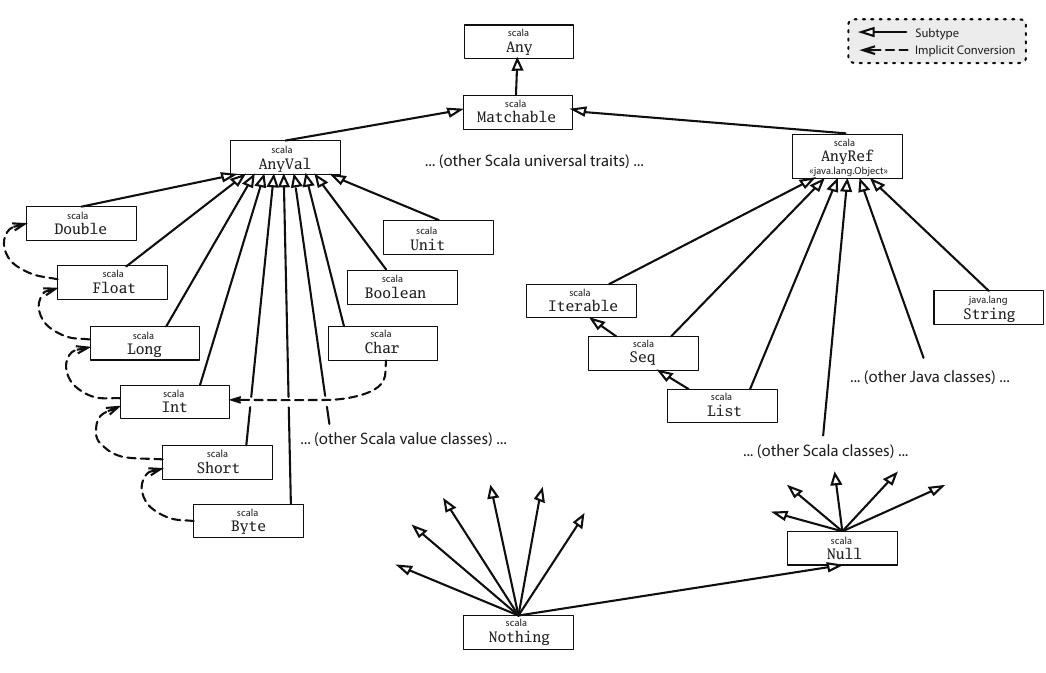
\includegraphics[width=.8\linewidth]{figures/scalaHierarchyWithMatchable.png}
    \caption{Scala type hierarchy with explicit nulls disabled.}
    \label{fig:scala-hierarchy-with-explicit-nulls-disabled}
\end{figure}

\begin{figure}
    \centering
    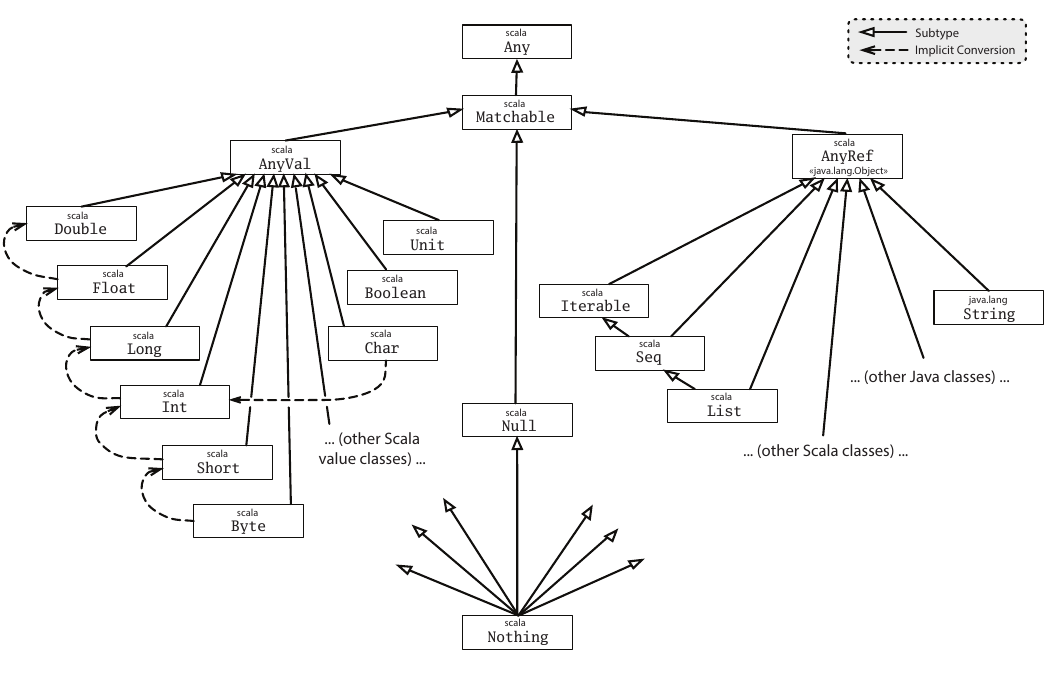
\includegraphics[width=.8\linewidth]{figures/scalaHierarchyWithMatchableAndSafeNull.png}
    \caption{Scala type hierarchy with explicit nulls enabled.}
    \label{fig:scala-hierarchy-with-explicit-nulls-enabled}
\end{figure}


\subsection{Multiversal Equality} \label{chap:background->sec:scala3->subsec:multiversal-equality}

Using context parameters of type \texttt{CanEqual[X, Y]}, the Scala 3 compiler with the \quotes{\texttt{-language:strictEquality}} flag enabled forbids universal equality, that allowed comparing any two values of any type, and replaces it with multiversal equality, which allows comparing any two values of any type, but only if the compiler can prove that the types are related by a \texttt{CanEqual} instance.
%
Implementing \texttt{CanEqual[X, Y]} instances can be automated with \textit{type class derivation}, a feature of Scala 3 that allows the compiler to synthesize given instances following rules defined by the user, often based on compositions of algebraic data types.
